\documentclass[12pt,a4paper]{article}
\usepackage[utf8]{inputenc}
\usepackage{xeCJK}
\setCJKmainfont{SimSun} % 可改为 Songti SC (Mac) 或其他字体
\usepackage{amsmath,amssymb,amsthm}
\usepackage{geometry}
\geometry{margin=1in}
\usepackage{hyperref}
\usepackage{enumitem}
\usepackage{listings}
\usepackage{xcolor}
\usepackage{mdframed}
\usepackage{graphicx}
\usepackage{float}
\lstset{
	language=C++,
	basicstyle=\ttfamily\small,
	keywordstyle=\color{blue},
	commentstyle=\color{gray},
	stringstyle=\color{red!70!black},
	numbers=left,
	numberstyle=\tiny,
	stepnumber=1,
	numbersep=5pt,
	tabsize=4,
	showspaces=false,
	showstringspaces=false,
	breaklines=true
}

\title{算法笔记}
\author{La5te2}
\date{\today}

\begin{document}
	
\maketitle
\tableofcontents
\makeatletter
\@addtoreset{section}{part} % 每次换 part,section 重置
\makeatother
\graphicspath{{image/}}


\newpage
\part{数论}
\section{数论基础}
\subsection{素性检测}
\subsection{质因数分解}
\subsection{数论函数}
\subsection{素数计数} % P7884 Meissel-Lehmer
\newpage
\section{欧拉函数}
\subsection{定义与性质}
\begin{mdframed}[leftline=true, linewidth=2pt, linecolor=gray]
	给定 $n\in \mathbf{N^*}$, 求 $\varphi(n)$.
\end{mdframed}
定义欧拉函数: \begin{equation*}\displaystyle\varphi(n)=\sum_{i=1}^{n}[\gcd(i,n)=1]\end{equation*}
通过算术基本定理有 $\displaystyle \varphi(n)=n\prod^{k}_{i=1}(1-\frac{1}{p_i})$,可证欧拉函数是积性函数,即
\begin{equation*}
	\gcd(n,m)=1\Rightarrow \varphi(nm)=\varphi(n)\varphi(m),\varphi(1)=1
\end{equation*}
通过莫比乌斯反演可以推出如下公式(欧拉反演):
\begin{equation*}
	n=\sum_{d\mid n}\varphi(d)
\end{equation*}
\subsection{欧拉定理}
\begin{mdframed}[leftline=true, linewidth=2pt, linecolor=gray]
	给定 $a,b,m\in \mathbf{N^*},\gcd(a,m)=1$, 求 $a^b\bmod{m}$.
\end{mdframed}
当 $\gcd(a,m)=1$ 时,若 $x_i$ 通过 $m$ 的简化系,则 $ax_i$ 通过 $m$ 的简化系,即\begin{equation*}
	\displaystyle\prod^{\varphi(m)}_{i=1}ax_i\equiv\prod^{\varphi(m)}_{i=1}x_i\pmod{m}
\end{equation*}
因为$\displaystyle\gcd(m,\prod^{\varphi(m)}_{i=1}x_i)=1$,有欧拉定理$a^{\varphi(m)}\equiv1\pmod{m}$,从而 $a^b\equiv a^{b\bmod{\varphi(m)}}\pmod{m}$
\subsection{扩展欧拉定理}
\begin{mdframed}[leftline=true, linewidth=2pt, linecolor=gray]
	给定 $a,b,m\in \mathbf{N^*}$,求 $a^b\bmod{m}$.
\end{mdframed}
对于本题,当 $b$ 小于 $\varphi(m)$ 时,直接做快速幂,否则有
\begin{equation*}
	\displaystyle a^b\equiv a^{b\bmod{\varphi(m)}+\varphi(m)}\pmod{m}
\end{equation*}
证明:当 $\gcd(a,m)=1$ 时,做法同1.2。\\
当$\gcd(a,m)\neq1$时,由算术基本定理,$\displaystyle a=\prod_{i=1}^{k}p_i^{e_i}$,即证 $p_i^b\equiv p_i^{r+\varphi(m)}\pmod{m}$。\\记 $p_i$ 为 $p$ ,若$\gcd(p,m)=1$,证明同1.2,否则有 $m\ge 2p$。\\
\\
令 $m=s\times p^t,t=\lfloor\log_p{m}\rfloor$,则 $\gcd(s,p^t)=\gcd(s,p)=1$,有
\begin{equation*}
	p^{\varphi(s)}\equiv1\pmod{s},\varphi(m)=\varphi(s)\varphi(p^t)\Rightarrow p^{\varphi(m)}=(p^{\varphi(s)})^{\varphi(p^t)}\equiv1\pmod{s}
\end{equation*}
两边同时乘以$p^t$,得到$p^{t+\varphi(m)}\equiv p^t\pmod{s\times p^t}$,即 $p^{t+\varphi(m)}\equiv p^t\pmod{m}$,从而
\begin{equation*}
	\displaystyle p^b=p^{b-t}\times p^t\equiv p^{b-t+t+\varphi(m)}=p^{b+\varphi(m)}\pmod{m}
\end{equation*}
记 $f(x)=p^{x}\bmod{m},x\ge\varphi(m)$,则 \begin{equation*}
	f(x+\varphi(m))=f(x)=f(x-\varphi(m))
\end{equation*}
又由定义域知 $x-\varphi(m)\ge\varphi(m)$,得 
\begin{equation*}
	f(x)=f(x\bmod{m}+\varphi(m))
\end{equation*}
即
\begin{equation*}
	p^b\equiv p^{b\bmod{\varphi(m)}+\varphi(m)}\pmod{m}\\
\end{equation*} 
\\得证。
\subsection{欧拉反演}
\subsection{欧拉筛}

\newpage
\section{阶与原根}
\subsection{性质与定理}
\begin{mdframed}[leftline=true, linewidth=2pt, linecolor=gray]
	给定 $n\in\mathbf{N^*}$,求它在 $[1,n)$ 中所有原根.
\end{mdframed}
由欧拉定理可知,满足 $a^n\equiv1\pmod m$ 的最小 $n\in\mathbf{N^*}$ 存在,称为 $a$ 模 $m$ 的阶,记作 $\delta_m(a)$。若 $\gcd(a,m)=1$ 且 $\delta_m(a)=\varphi(m)$,称 $a$ 为模 $m$ 的原根。\\
\\
阶的三条性质:
\begin{enumerate}
	\item 若 $a^n\equiv 1\pmod m$,则 $\delta_m{(a)}\mid n$
	\item 设 $m\in \mathbf{N}^*,a,b\in\mathbf{Z},\gcd(a,m)=\gcd(b,m)=1$,则 \begin{equation*}
		\delta_m(ab)=\delta_m(a)\delta_m(b)\iff \gcd(\delta_m(a),\delta_m(b)=1)
	\end{equation*}
	\item 设 $k\in\mathbf{N},m\in\mathbf{N^*},a\in\mathbf{Z}, \gcd(a,m)=1$,则 $\displaystyle\delta_m(a^k)=\frac{\delta_m(a)}{\gcd(\delta_m(a),k)}$
\end{enumerate}
拉格朗日定理:设 $p$ 为素数,对于模 $p$ 意义下的整系数多项式 
\begin{equation*}
	f(x)=a_nx^n+a_{n-1}x^{n-1}+\cdots+a_0\;(p\nmid a_n)
\end{equation*}
同余方程 $f(x)\equiv 0\pmod p$ 在模 $p$ 意义下至多有 $n$ 个不同解。当 $n=0$ 时显然成立。\\若命题对于 $\deg f< n$ 的 $f$ 都成立,反设存在一个满足题目条件的 $f$ 在模 $p$ 意义下有着至少 $n+1$ 个不同的解 $x_0,x_1,\cdots,x_{n}$,可设
\begin{equation*}
	f(x)-f(x_0)=(x-x_0)g(x)
\end{equation*}
则 $g(x)$ 在模 $p$ 意义下 $\deg g<n$,至多有 $n-1$ 个解,且对于 $i\in[1,n]$,有 
\begin{equation*}
	(x_i-x_0)g(x_i)\equiv f(x_i)-f(x_0)\equiv0\pmod p
\end{equation*}
又 $x_i\not\equiv x_0\pmod p$,故 $g(x_i)\equiv0\pmod p$,从而 $g(x)\equiv0\pmod p$ 有至少 $n$ 个根,矛盾。所以,命题对 $n$ 次多项式也成立,定理获证。\\
\\
原根存在定理: $m=1,2,4,p,p^\alpha,2p^\alpha$,其中 $p$ 为奇素数,$\alpha\in\mathbf{N^*}$。
\\
\\
\textbf{命题1: 奇素数 $p$ 有原根.}
\\引理:设 $a, b\in\mathbf{Z},\gcd(a,p)=\gcd(b,p)=1$,则存在 $c\in\mathbf{Z}$ 使得 \begin{equation*}
	\delta_p(c)=lcm(\delta_p(a),\delta_p(b))
\end{equation*}
由算术基本定理(非严格,$\max(\alpha_j,\beta_j)>0$),有 
\begin{equation*}
	\displaystyle \delta_p(a)=\prod_{j=1}^{s}p_j^{\alpha^{j}},\delta_p(b)=\prod_{j=1}^{s}p_j^{\beta^{j}}
\end{equation*}
令 $\displaystyle l=\prod_{j=1}^{s}p_j^{\alpha^{j}}[\alpha_j\le\beta_j],n=\prod_{j=1}^{s}p_j^{\alpha^{j}}[\alpha_j>\beta_j]$,记 $r=lx,t=ny$,则 \begin{equation*}
	\gcd(x,y)=1,\operatorname{lcm}(r,t)=xy
\end{equation*}
由阶的性质3,\begin{equation*}
	\displaystyle\delta_p(a^l)=x,\delta_p(b^n)=y
\end{equation*}
再由阶的性质2,
\begin{equation*}
	\displaystyle\delta_p(c)=\delta_p(a^lb^n)=xy=\operatorname{lcm}(\delta_p(a),\delta_p(b))
\end{equation*}
回到原命题,对 $1\sim(p-1)$ 依次两两使用上述引理,可知存在 $g\in\mathbf{Z}$ 使得 
\begin{equation*}
	\delta_p(g)=\operatorname{lcm}\left(\delta_p(1),\delta_p(2),\cdots,\delta_p(p-1)\right)
\end{equation*}
这表明 
\begin{equation*}\delta_p(j)|\delta_p(g),j=1,2,\cdots,p-1\end{equation*}
所以 $j=1,2...,p-1$ 都是方程 $x^{\delta_p(g)}\equiv1\pmod p$ 的根,由拉格朗日定理可知方程次数 $\delta_p(g)\ge p-1$,又由费马小定理可知 $\delta_p(g)\le p-1$,所以 $\delta_p(g)=p-1=\varphi(p)$。
综上,$g$ 为模 $p$ 的原根,奇素数都存在原根。
\\
\\
\textbf{命题2: $p^{\alpha}$ 有原根.}
\\引理1:存在模 $p$ 的原根 $g$,使得 $g^{p-1}\not\equiv1\pmod{p^2}$。

设 $g$ 为模 $p$ 的原根,易证 $g+kp$ 也是模 $p$ 的原根。若 $g^{p-1}\equiv1\pmod{p^2}$,则 
\begin{equation*}
	(g+p)^{p-1}\equiv C^0_{p-1}g^{p-1}+C^1_{p-1}pg^{p-1}\equiv1+p(p-1)g^{p-2}\not\equiv1\pmod{p^2}
\end{equation*}
\\引理2:若选取满足引理1的原根 $g$,对于 $\forall l\in\mathbf{N^*}$,均有 
\begin{equation*}
	g^{\varphi(p^l)}=1+p^l\times k,p\nmid k
\end{equation*}

归纳法:$l=1$ 时由 $g$ 的选取结论显然成立,假设上式对 $l$ 时成立,则 
\begin{equation*}
	g^{\varphi(p^{l+1})}=(g^{\varphi(p^l)})^p=(1+p^l\times k)^p\equiv1+p^{l+1}\times k\pmod{p^{l+2}}
\end{equation*}
结合 $p\nmid k$ 可知引理2对 $l+1$ 成立,得证。

回到原命题,满足引理1的原根 $g$ 是模 $p^\alpha$ 的原根,证明如下:

记 $\delta=\delta_{p^\alpha}(g)$,由欧拉定理和阶的性质,可知 
\begin{align*}
	\delta\mid\varphi(p^\alpha)=p^{\alpha-1}(p-1)\\ g^\delta\equiv1\pmod{p^\alpha}
\end{align*}
故 $\varphi(p)=p-1\mid \delta$,可设 $\delta=p^{\beta-1}(p-1),1\le\beta\le \alpha$。由引理2,有 \begin{equation*}
	g^{\varphi(p^{\beta})}\not\equiv 1\pmod {p^{\beta+1}}\Rightarrow g^{\delta}\not\equiv 1\pmod {p^{\beta+1}}
\end{equation*}结合 $g^\delta\equiv1\pmod{p^\alpha}$ 可知 $\beta\ge \alpha$。综上,$\beta=\alpha$,即 
\begin{equation*}
	\delta=p^{\alpha-1}(p-1)=\varphi(p^\alpha)
\end{equation*}从而 $g$ 是模 $p^\alpha$ 的原根。
\\
\\\textbf{命题3: $2p^\alpha$ 有原根.}

记 $G$ 是模 $p^\alpha$ 的奇数原根,$\delta=\delta_{2p^\alpha}(G)$,则 $\gcd(G, 2p^\alpha)=1$。由欧拉定理,$\delta\mid \varphi(2p^\alpha)$。而 $G^\delta\equiv1\pmod{2p^\alpha}$,故 $G^\delta\equiv1\pmod{p^\alpha}$,结合 $G$ 是模 $p^\alpha$ 的原根可知 $\varphi(p^\alpha)\mid \delta$,所以 $\delta=\varphi(p^\alpha)=\varphi(2p^\alpha)$,即 $G$ 是模 $2p^\alpha$ 的原根。
\\
\\\textbf{命题4: 若 $m\neq 1,2,4,p^\alpha,2p^\alpha$,则对任意 $a\in\mathbf{Z},\gcd(a,m)=1$,都有 $\delta_m(a)<\varphi(m)$}。

若 $m=2^\alpha,\alpha\in\mathbf{N^*},\alpha\ge3$,对于任意偶数均有 $\gcd(2k,m)\ne1$,对于任意奇数 $a=2k+1$,
公式
\begin{align*}
	a^{2^{\alpha-2}}
	&=(2k+1)^{2^{\alpha-2}}\\
	&\equiv1+C_{2^{\alpha-2}}^1(2k)+C_{2^{\alpha-2}}^{2}(2k)^2+0\\
	&\equiv1+2^{\alpha-1}k+2^{\alpha-1}(2^{\alpha-2}-1)k^2\\
	&\equiv 1+2^{\alpha-1}(k+(2^{\alpha-2}-1)k^2)\\
	&\equiv 1 \pmod {2^{\alpha}}
\end{align*}
而 $2^{\alpha-2}<\varphi(m)=2^{\alpha-1}$。

若 $m$ 不是 $2$ 的幂,可设 $m=rt,2<r<t,\gcd(r,t)=1$,由欧拉定理可知 
\begin{equation*}
	a^{\varphi(r)}\equiv1\pmod r,a^{\varphi(t)}\equiv1\pmod t
\end{equation*}
注意到 $n>2$ 时 $2\mid\varphi(n)$,所以 
\begin{align*}
	\displaystyle a^{\frac{1}{2}\varphi(r)\varphi(t)}\equiv1\pmod{r}\\
	a^{\frac{1}{2}\varphi(r)\varphi(t)}\equiv1\pmod{t}
\end{align*}
用 \textbf{CRT} 求通解得到 
\begin{equation*}
	\displaystyle a^{\frac{1}{2}\varphi(r)\varphi(t)}\equiv1\pmod{rt}
\end{equation*}
进而有如下不等式:$\displaystyle\delta_m(a)\le\frac{1}{2}\varphi(r)\varphi(t)=\frac{1}{2}\varphi(rt)=\frac{1}{2}\varphi(m)<\varphi(m)$。

综上,若 $m\neq 1,2,4,p^\alpha,2p^\alpha$,则对任意 $a\in\mathbf{Z},\gcd(a,m)=1$,都有 $\delta_m(a)<\varphi(m)$,即模 $m$ 的原根不存在。

由原根的定义,若 $g$ 为模 $m$ 的原根,则对于 $\varphi(m)$ 的任意素因数 $p$,必有 
\begin{equation*}
	g^{\varphi(m)/p}\not\equiv1\pmod{m}
\end{equation*}
且 $g^{\varphi(m)}\equiv1\pmod m$。反之,由 $\delta\mid\varphi$,满足上述条件的 $g$ 必定是模 $m$ 的原根。

假设正整数 $n$ 的一个原根是 $g$,由阶的性质3可知,任意满足 $\gcd(x,\varphi(n))=1$ 的 $x$,$g^x$ 都是模 $n$ 的原根,从而模 $n$ 意义下一共有 $\varphi(\varphi(n))$ 个原根。可以证明在 $[1,n)$ 中的最小原根 $g_n=O(n^{0.25+\epsilon})$。

综上,预处理出 $\varphi(n)$ 的所有素因数,从小到大枚举 $g$,快速幂来判断是否是原根,找到最小原根后再枚举所有满足条件的 $g^x$ 即可。代码如下:
\begin{lstlisting}
int MPR(int n, int p, int l, int r) { // minimum primitive root
	int q = p; // EulerSieve first, p = phi[n]
	std::vector<int> pri;
	for(int i = 2; i * i <= q; i++) {
		if(q % i == 0) pri.push_back(i);
		while(q % i == 0) q /= i;
	} if(q > 1) pri.push_back(q);
	auto check = [&](int i) -> bool {
		if(qpow(i, p, n) != 1) return 0;
		for(auto j : pri) if(qpow(i, p / j, n) == 1) return 0;
		return 1;
	}; // l = 1, r = 50
	for(int i = l; i <= r; i++) if(check(i)) return i;// n^0.25
	return 0;
}
\end{lstlisting}
\subsection{Carmichael函数}
\begin{mdframed}[leftline=true, linewidth=2pt, linecolor=gray]
	求使得同余关系 $a^n\equiv 1\pmod{m}$ 对所有 $\gcd(a,m)=1$ 都成立的最小正整数 $n$. 
\end{mdframed}
\newpage
\section{Euclid算法}
\subsection{扩展Euclid算法} %包括辗转相除法
\subsection{类Euclid算法}
\newpage
\section{同余方程}
\subsection{裴蜀定理}
\subsection{多元不定方程}
\subsection{线性同余方程}
\subsection{模逆元筛}
\subsection{CRT定理}
\subsection{扩展CRT定理}
\subsection{阶乘取模}
\subsection{N次同余方程}
\newpage
\section{离散对数和剩余}
\subsection{BSGS算法}
\begin{mdframed}[leftline=true, linewidth=2pt, linecolor=gray]
	给定质数 $p$, $a,b\in \mathbf{Z}$,计算最小的 $l\in\mathbf{N}$,满足 $a^l \equiv b \pmod p$.
\end{mdframed}

由 $\gcd(a,p)=1$,在模 $p$ 意义下可以直接执行关于 $a$ 的乘除运算。

由扩展欧拉定理,$a^i$在模$p$意义下会出现循环节$c$且 $c|\varphi(p)$。可知对于原方程 \begin{equation*}
	a^l \equiv b \pmod p
\end{equation*}
至多枚举$\varphi(p)$个数就能知道方程的解或无解,从而 $l\leq p$。

令 $m=\lceil\sqrt{p}\rceil$,$l=i\times m-j$,$i\in[1,m],j\in[0,m)$,$A=a^m\bmod{p}$,原方程变形为 \begin{equation*}
	A^i\equiv ba^j\pmod{p}
\end{equation*}
枚举 $ba^j$ 并将结果存入哈希表,再枚举 $A^i$,如果枚举到 $i=i_0\in [1,m]$ 时有 
\begin{equation*}
	A^{i_0}\in hash
\end{equation*}
说明存在 $j$ 使得 \begin{equation*}
	hash[A^{i_0}]=hash[ba^j]=j
\end{equation*}
答案为 $l=i_0\times m-j$。按照顺序枚举,可以保证$hash[ba^j]$对应得$j$最大,$i_0$最小,从而保证 $l$ 是最小非负整数。

\subsection{扩展BSGS算法}
\begin{mdframed}[leftline=true, linewidth=2pt, linecolor=gray]
	给定 $a,b,m\in \mathbf{Z}$,计算最小的 $X\in\mathbf{N}$,满足 $a^X \equiv b \pmod m$.
\end{mdframed}

若 $\gcd(a,m)\ne1$,不能直接使用\textbf{BSGS},考虑将原方程化为\begin{equation*}
	(a')^{Y}\equiv b'\pmod{m'},\gcd(a',m')=1
\end{equation*}

原方程等价于
\begin{equation*}
	a\cdot a^{X-1}+my=b
\end{equation*}
令 $d_1=\gcd(a,m)$,由裴蜀定理知,方程有解当且仅当 $d_1\mid b$,因此方程两边同除以 $d_1$:
\begin{equation*}
	\displaystyle\frac{a}{d_1}\cdot a^{X-1}+\frac{m}{d_1}y=\frac{b}{d_1}
\end{equation*}
如果此时 $\displaystyle d_2=\gcd(a,\frac{m}{d_1})\neq 1, d_2\mid\frac{b}{d_1}$,方程两边同除以 $d_2$,得到 \begin{equation*}
	\displaystyle\frac{a^2}{d_1d_2}\cdot a^{X-2}+\frac{m}{d_1d_2}y=\frac{b}{d_1d_2}
\end{equation*}

重复此过程,直到 $\displaystyle\gcd(a, \frac{m}{d_1d_2...d_k})=1$,令 $D=d_1d_2...d_k$,原方程等价于
\begin{equation*}
	\displaystyle \frac{a^k}{D}\cdot a^{X-k}\equiv\frac{b}{D}\ (mod\ \frac{m}{D})
\end{equation*}
此时应用\textbf{BSGS}即可。
\newpage
\subsection{离散对数筛}
\begin{mdframed}[leftline=true, linewidth=2pt, linecolor=gray]
	给定质数 $p$ 以及正整数 $g$,有 $q$ 组询问,每组询问给出整数 $y$,找到最小的 $x\in\mathbf{N^*}$ 使得 $g^x\equiv y\pmod p$.
\end{mdframed}
假设对每一组询问单独运行\textbf{BSGS},时间复杂度为 $O(q\sqrt{p})$,不能够通过本题。\\
\\
不妨设 $g$ 是模 $p$ 的原根,则 $x=ind(y)$ 一定有解。\\
考虑欧拉筛,记 $\pi(n)$为 $n$ 及以内素数的个数,利用离散对数与对数相似的性质:
\begin{equation*}
	ind(ab)\equiv ind(a)+ind(b)\pmod{\varphi(p)}
\end{equation*}
只需要求 $\pi(n)$ 个离散对数就可以通过欧拉筛线性求出 $n$ 及以内剩下的数的离散对数。令 $x=ind(y)=i\times B+j,x\in[0,p),0\le j< B,0\le i\le\lfloor(p-1)/B\rfloor$,有
\begin{equation*}
	g^j\equiv y\times g^{-B}\pmod p
\end{equation*}
枚举 $j\in[0,B)$,将 $g^j$ 插入哈希表,接着枚举 $\displaystyle i\in[0,\frac{p}{B}]$,查询时间复杂度为 $O(\pi(n)p/B)$,则求离散对数总时间复杂度为 $O(B+\pi(n)p/B)$,令 $B=\sqrt{\pi(n)p}$ 最优。\\
同时为了使单次询问复杂度尽可能小,取 $n=\sqrt{p}+1$,从而可以 $O(1)$ 回答 $\sqrt{p}+1$以内的离散对数值,对于 $y\in(\sqrt{p}+1,p)$ 的询问,考虑迭代。设当前要回答 $ind(a)$,则可令 $p=ba+c,b\le\sqrt{p},c=p\bmod a$,发现 $ind(b),ind(b+1)$ 可以直接得到,考虑转化式子:
\[\begin{cases}
	a=\dfrac{p-c}{b} 
	&\Rightarrow \operatorname{ind} a \equiv \operatorname{ind}(-c)-\operatorname{ind} b 
	\equiv \operatorname{ind}(-1)+\operatorname{ind} c-\operatorname{ind} b, \\[6pt]
	a=\dfrac{p+a-c}{b+1} 
	&\Rightarrow \operatorname{ind} a \equiv \operatorname{ind}(a-c)-\operatorname{ind}(b+1).
\end{cases}\]
因为有 $min(c,a−c)\le2a$,每次递归都会折半,故单次查询复杂度为 $O(\log p)$,总时间复杂度约为 $O(\sqrt{\pi(\sqrt{p})p}+q\log{p})$。\\
\\
若 $g$ 不是模 $p$ 的原根,考虑换底公式。令 $h$ 是模 $p$ 的原根,对 $h$ 运行离散对数筛。假设询问以 $g$ 为底 $y$ 的离散对数,令 $k=ind_h(g),t=ind_h(y)$。由定义知:
\begin{equation*}
	h^k\equiv g,h^t\equiv y,g^x\equiv y\Rightarrow h^{kx}\equiv h^t\pmod{p}
\end{equation*}
从而 $kx\equiv t\pmod{\varphi(p)}$。解同余方程:若 $d=\gcd(k,\varphi(p))\nmid t$ 则无解,否则令$\displaystyle k'=\frac{k}{d},t'=\frac{t}{d},M=\frac{\varphi(p)}{d}$, $ind_2(y)\equiv t'\cdot (k')^{-1}\pmod M$。
\subsection{剩余}
\subsection{二次剩余}

\newpage
\section{数论分块}
\subsection{引理与结论}
\subsection{N维数论分块}
\begin{mdframed}[leftline=true, linewidth=2pt, linecolor=gray]
	求值:$\displaystyle(\sum_{i=1}^{n} \sum_{j=1}^{m} (n \bmod i) \times (m \bmod j))\bmod{19940417},i \neq j,1 \leq n,m \leq 10^9$
\end{mdframed}
不妨设 $n\le m$,由于 $i\ne j$,原式等价于 \begin{equation*}
	\displaystyle(\sum_{i=1}^{n} \sum_{j=1}^{m} (n \bmod i) \times (m \bmod j)-\sum_{i=1}^{n}(n \bmod i) \times (m \bmod i))\bmod{19940417}
\end{equation*}
又 $\displaystyle a\bmod b=a-\lfloor\frac{a}{b}\rfloor\times b$,故原式可以展开为:
\begin{align*}
	\displaystyle Ans &= 
	\sum_{i=1}^{n} \sum_{j=1}^{m} (n \bmod i) \times (m \bmod j)
	- \sum_{i=1}^{n} (n \bmod i) \times (m \bmod i) \\[1mm]
	&= \sum_{i=1}^{n} (n \bmod i) \times \sum_{j=1}^{m} (m \bmod j)
	- \sum_{i=1}^{n} (n \bmod i) \times (m \bmod i) \\[1mm]
	&= \sum_{i=1}^{n} \bigl(n - \lfloor \frac{n}{i} \rfloor \cdot i \bigr)
	\times \sum_{j=1}^{m} \bigl(m - \lfloor \frac{m}{j} \rfloor \cdot j \bigr)
	- \sum_{i=1}^{n} \bigl(n - \lfloor \frac{n}{i} \rfloor \cdot i \bigr)
	\times \bigl(m - \lfloor \frac{m}{i} \rfloor \cdot i \bigr) \\[1mm]
	&= \bigl[n^2 - \sum_{i=1}^{n} \lfloor \frac{n}{i} \rfloor \cdot i \bigr]
	\bigl[m^2 - \sum_{j=1}^{m} \lfloor \frac{m}{j} \rfloor \cdot j \bigr] 
	- \sum_{i=1}^{n} \Bigl(nm - m i \cdot \lfloor \frac{n}{i} \rfloor - n i \cdot \lfloor \frac{m}{i} \rfloor + \lfloor \frac{n}{i} \rfloor \lfloor \frac{m}{i} \rfloor \cdot i^2 \Bigr)
\end{align*}
对于形如 $\displaystyle \sum_{i=1}^{n}(\lfloor\frac{n}{i}\rfloor\times f(i))$ 的求和式,使用整除分块。注意到 $\displaystyle\lfloor\frac{n}{i}\rfloor$ 为一个不下降子序列,且呈块状分布。\\

对于每个以 $l$ 为起点的块,块中每一个元素的值都是 $\displaystyle t=\lfloor\frac{n}{l}\rfloor$,块的终点为 $\displaystyle r=\lfloor\frac{n}{t}\rfloor$,因此可以 $O(1)$ 计算块中元素的和,从而 $O(T\sqrt{n})$ 计算 $\displaystyle\sum_{i=1}^{n}(\lfloor\frac{n}{i}\rfloor\times f(i))$,其中 $T$ 取决于计算 $\displaystyle \sum_{i=l}^{r}f(i)$ 的复杂度。

对于 $\displaystyle \sum_{i=1}^{N}(\lfloor\frac{n}{i}\rfloor\lfloor\frac{m}{i}\rfloor\times f(i)),N=\min(n,m)$,同样考虑整除分块,对于每个以 $l$ 为起点的块,令 $\displaystyle t_1=\lfloor\frac{n}{l}\rfloor,t_2=\lfloor\frac{m}{l}\rfloor$,块的终点为 $\displaystyle r=\min(\lfloor\frac{n}{t_1}\rfloor,\lfloor\frac{n}{t_2}\rfloor)$,块中元素和为 $\displaystyle \prod_{i=1}^{k=2}t_i\times \sum_{i=l}^{r}f(i)$。该方法可以推广至 $k$ 维整除分块:$\displaystyle \sum_{i=1}^{N}(\prod_{j=1}^{k}\lfloor\frac{n_j}{i}\rfloor\times f(i)),N=\min\{n_j\}$。

注:$N=\min\{n_j\}$ 的原因在于当 $i>N$ 时至少有一个 $\displaystyle\lfloor\frac{n_j}{i}\rfloor$ 为 $0$,则和为 $0$,可以忽略;同时排除 $t_j=0$ 的情况,避免除以 $0$。
\subsection{向上取整}
\subsection{扩展数论分块}
\newpage
\section{Dirichlet卷积}
\subsection{Dirichlet前缀和}
\begin{mdframed}[leftline=true, linewidth=2pt, linecolor=gray]
	给定数列 $\{a_n\}$。求出数列 $\{b_n\}$,满足 $\displaystyle b_k=\sum_{i|k}a_i$。$1\leq n\leq 2\times 10^7$,$0\leq a_i< 2^{32}$
\end{mdframed}

首先介绍求解 $k$ 维前缀和的一般方法。给定 $k$ 维数组 $A$,大小为 $\displaystyle N=\prod_{i=1}^{k}{N_i}$,求其前缀和 $S$。若采用容斥原理,时间复杂度为 $O(N\times2^k)$,当 $k$ 较大时不够优秀。\\

对于一般的情形,可以将 $S$ 表示为:
\begin{equation*}
	\displaystyle S_{i_1\cdots i_k}=\sum_{i'_1\le i_1}\cdots\sum_{i'_k\le i_k}A_{i'_1\cdots i'_k}
\end{equation*}
注意到 $k$ 维前缀和等价于进行 $k$ 次求和。因此每次只考虑一个维度,固定所有其它维度,然后对 $k$ 个维度分别求一维前缀和,得到的就是 $k$ 维前缀和。这种方法称为逐维前缀和,其时间复杂度为 $O(kN)$。

逐维前缀和可以解决一类问题:考虑大小为 $n$ 的集合的全体子集上定义的函数 $f$,求出其子集和函数 $g$,满足
\begin{equation*}
	\displaystyle g(S)=\sum_{T\subseteq S}f(T)
\end{equation*}
即 $g(S)$ 等于其所有子集 $T\subseteq S$ 上的函数值 $f(T)$ 的和,称其为子集和问题。

如果用朴素的子集枚举求解,复杂度为 $\displaystyle O(\sum_{i=1}^{n}\mathbf{C}_{n}^{i}\cdot2^n=3^n)$,而应用逐维前缀和可以达到 $O(n\cdot2^n)$。首先,将子集和问题表示为高维前缀和的形式:注意到 $S$ 的子集可以通过状态压缩的思想表示为长度为 $n$ 的二进制数 $s$,将其每一位都看作数组下标的一个维度,则 $f$ 就是一个 $n$ 维数组,且每个下标状态都是 $\{0,1\}$,即 $N=2^n$。同时,子集的包含关系等价于下标的大小关系,即 $T\subseteq S\iff\forall i(t_i\le s_i)$。因此子集和问题等价于 $n$ 维前缀和。

\begin{lstlisting}
for(int i = 0; i < n; i++) 
	for(int j = 0; j < (1 << i); j++) 
		if((j >> i) & 1) f[j] += f[j ^ (1 << i)]; // g = f
\end{lstlisting}
回到原题,考虑对 $b_k$ 产生贡献的 $a_i$,则有 $i\mid k$,由算数基本定理,令 \begin{equation*}
	\displaystyle i=\prod_{p\in\mathcal{P}}p_j^{\alpha_j},k=\prod_{p\in\mathcal{P}}p_j^{\beta_j}
\end{equation*}
则 $\forall j(\alpha_j\le\beta_j)$ 成立,因此原问题等价于 $\displaystyle b_k=\sum_{I\subseteq K}a_i$,其中 $I$ 表示 $i$ 分解出的质数可重集合,$K$ 表示 $k$ 分解出的质数可重集合。对于单个的 $k$ 而言,子集枚举的维度数为 $K$ 中元素的种类数,每个维度的状态数都是 $K$ 中对应元素的数量,$K$ 的子集($k$ 的约数集)可以通过筛法得到。考虑埃氏筛,对于 $n$ 以内每一个质数 $p$,标记其所有合数 $k$ 的同时将 $k$ 的约数 $j$ 对应的 $a_j$ 累加进 $a_k$, 总的维度数为 $\pi(n)$,从而 $\displaystyle b_k=a'_k=\sum_{I\subseteq K}a_i$,时间复杂度为 $O(n\log\log n)$。

\begin{lstlisting}
for(int i = 2;i <= n; i++) if(!vis[i])/*pi(n)*/ 
	for(int k = i, j = 1; k <= n; k += i, j++) 		
		a[k] += a[j], vis[k] = 1; // b = a
	
\end{lstlisting}
更直观地,假设已经筛出了 $1\sim n$ 的所有质数,记第 $i$ 个质数为 $p_i$,共有 $tot$ 个质数:

\begin{lstlisting}
for(int i = 1; i <= tot; i++)
	for(int d = 1; p[i] * d <= n; d++)
		a[p[i] * d] += a[d]; // b=a
	
\end{lstlisting}
这个过程称为 \textbf{Dirichlet} 前缀和。

\subsection{Dirichlet后缀和}
\begin{mdframed}[leftline=true, linewidth=2pt, linecolor=gray]
	给定正整数数列 $\{a_n\}$,设它的一个排列 $p$ 的权值为 $w=\displaystyle \sum_{i=1}^{n}\gcd(a_1,\cdots,a_i)$,求 $w$ 的最大值。$1\le n\le10^5,1\le a_i\le2\times10^7$
\end{mdframed}
\subsection{DGF与卷积}

\newpage
\section{积性函数筛}

\newpage
\section{莫比乌斯函数}

\newpage
\part{图论} % 包括树论
\section{最短路问题}
\newpage
\section{生成树问题}
\newpage
\section{连通性问题}
\newpage
\section{网络流}
\subsection{基本定义}
给定有源汇网络 $(G,s,t)$,定义容量函数和流函数 $c,f:\mathbf{E}\rightarrow\mathbb{Z}|\mathbb{R}$,其满足如下条件:
\begin{itemize}
	\item 容量限制:$f(u,v)\le c(u,v)$,等号成立时称为满流,$f(u,v)=0$ 时称空流。
	\item 斜对称:$f(u,v)=-f(v,u)$,$(v,u)$ 为反向边,$(u,v)\in\mathbf{E}^+,(v,u)\in\mathbf{E}^-$。
	\item 流量守恒:$\displaystyle\forall u(u\in \mathbf{V},u\ne s,u\ne t)$,净流量为 $0$(边不存在时 $f=0$):
	\begin{equation*}
		f(u)=\sum_{v\in\mathbf{V}}f(u,v)-\sum_{v\in\mathbf{V}}f(v,u)=0
	\end{equation*}
\end{itemize}
有源汇网络的相关定义如下:
\begin{itemize}
	\item 根据斜对称和流量守恒,有 $|f|=f(s)=-f(t)$,称为当前流 $f$ 的流量。最大流量为所有合法 $f$ 中 $|f|$ 的最大值。
	\item 定义流 $f$ 在网络 $G$ 上的残量网络 $G_f=(\mathbf{V},\mathbf{E}_f)$ 为容量函数 $c_f=c-f$ 的网络。根据容量限制,有 $c_f(u,v)\ge0$,等号成立时视 $(u,v)$ 在 $G_f$ 上不存在。
	\item 定义增广路为残量网络 $G_f=(\mathbf{V},\mathbf{E}_f)$ 上一条从源点 $s$ 到汇点 $t$ 的路径。
	\item 将 $\mathbf{V}$ 分成不相交的两个点集 $S,T$ 且 $s\in S, t\in T$,这种划分方式称为 $s-t$ 割,定义其容量为 $\displaystyle c_c=\sum_{u\in S}\sum_{v\in T}c(u,v)$,流量为 $\displaystyle f_c=\sum_{u\in S}\sum_{v\in T}f(u,v)$。
	\item 当 $u,v$ 属于不同点集时,称 $(u,v)$ 为割边。当 $c_c$ 最小时称最小割,记为 $\|S,T\|$。
\end{itemize}
\subsection{最大流}
\begin{mdframed}[leftline=true, linewidth=2pt, linecolor=gray]
	给定网络 $G=(\mathbf{V}, \mathbf{E})$ 和源汇点,求最大流量(Max Flow)。
\end{mdframed}
\subsubsection{Ford–Fulkerson增广}
考虑贪心:找到残量网络 $G_f$ 上的一条增广路 $P$ 并为 $P$ 上每一条边增加 $\displaystyle c_f(P)=\min_{(u,v)\in P}c_f(u,v)$ 的流量,此过程称为增广,重复增广直到 $G_f$ 上不存在增广路。\\\\
显然,如果增加的流量大于该值,一些边将不满足容量限制,而根据能流满就流满的思想,增加的流量也不应小于该值。这种贪心不一定是正确的,考虑下图:
\begin{figure}[H]
	\centering
	% \raggedright
	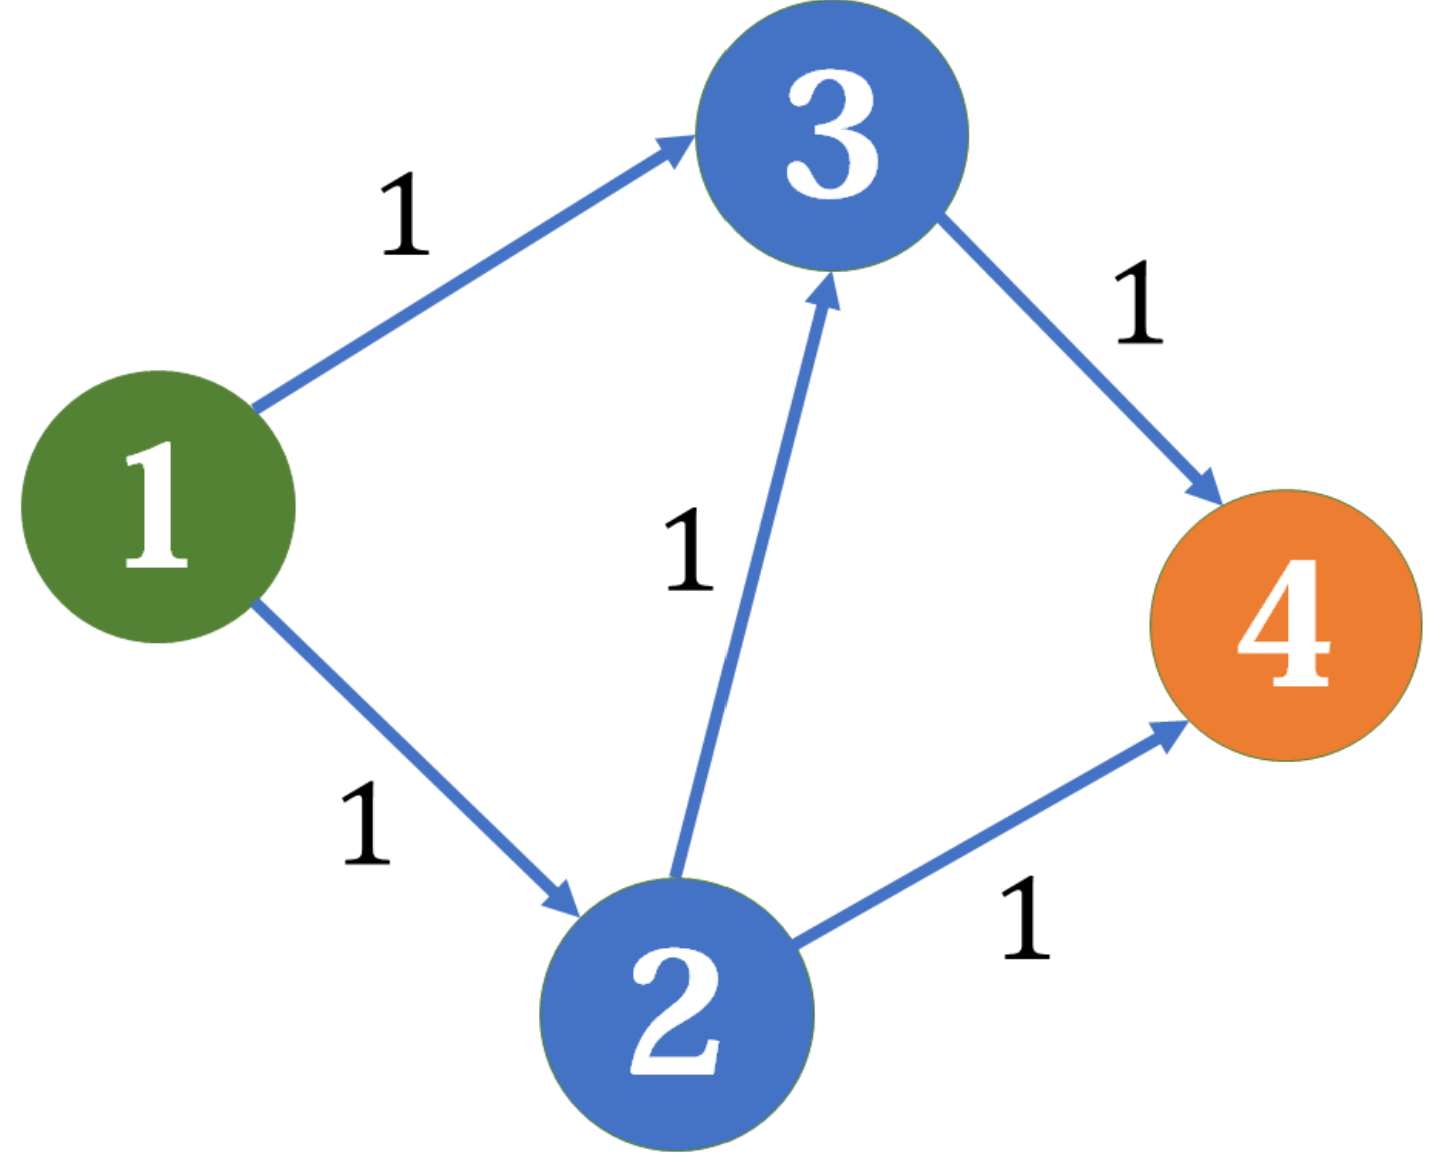
\includegraphics[width=0.3\textwidth]{maxflow1.png}
	% \caption{(1)}
	% \label{fig:example}
\end{figure}
\noindent 令 $s=1, t=4$,首先选择增广路 $(1,2,3,4)$ 会导致残量网络上没有其他的增广路,从而 $|f|=1$,但实际上的最大流为选择增广路 $(1,3,4)$ 和 $(1,2,4)$,此时 $|f|=2$。\\
为了保证正确性,对每条边建立满足斜对称且能快速访问的反向边,目的是支持反悔。\\
具体地,在为当前边 $(u,v)\in P$ 增加流量 $c_f(P)$ 时,给其反边 $(v,u)$ 的容量加上 $c_f(P)$。\\
\begin{figure}[H]
	\centering
	% \raggedright
	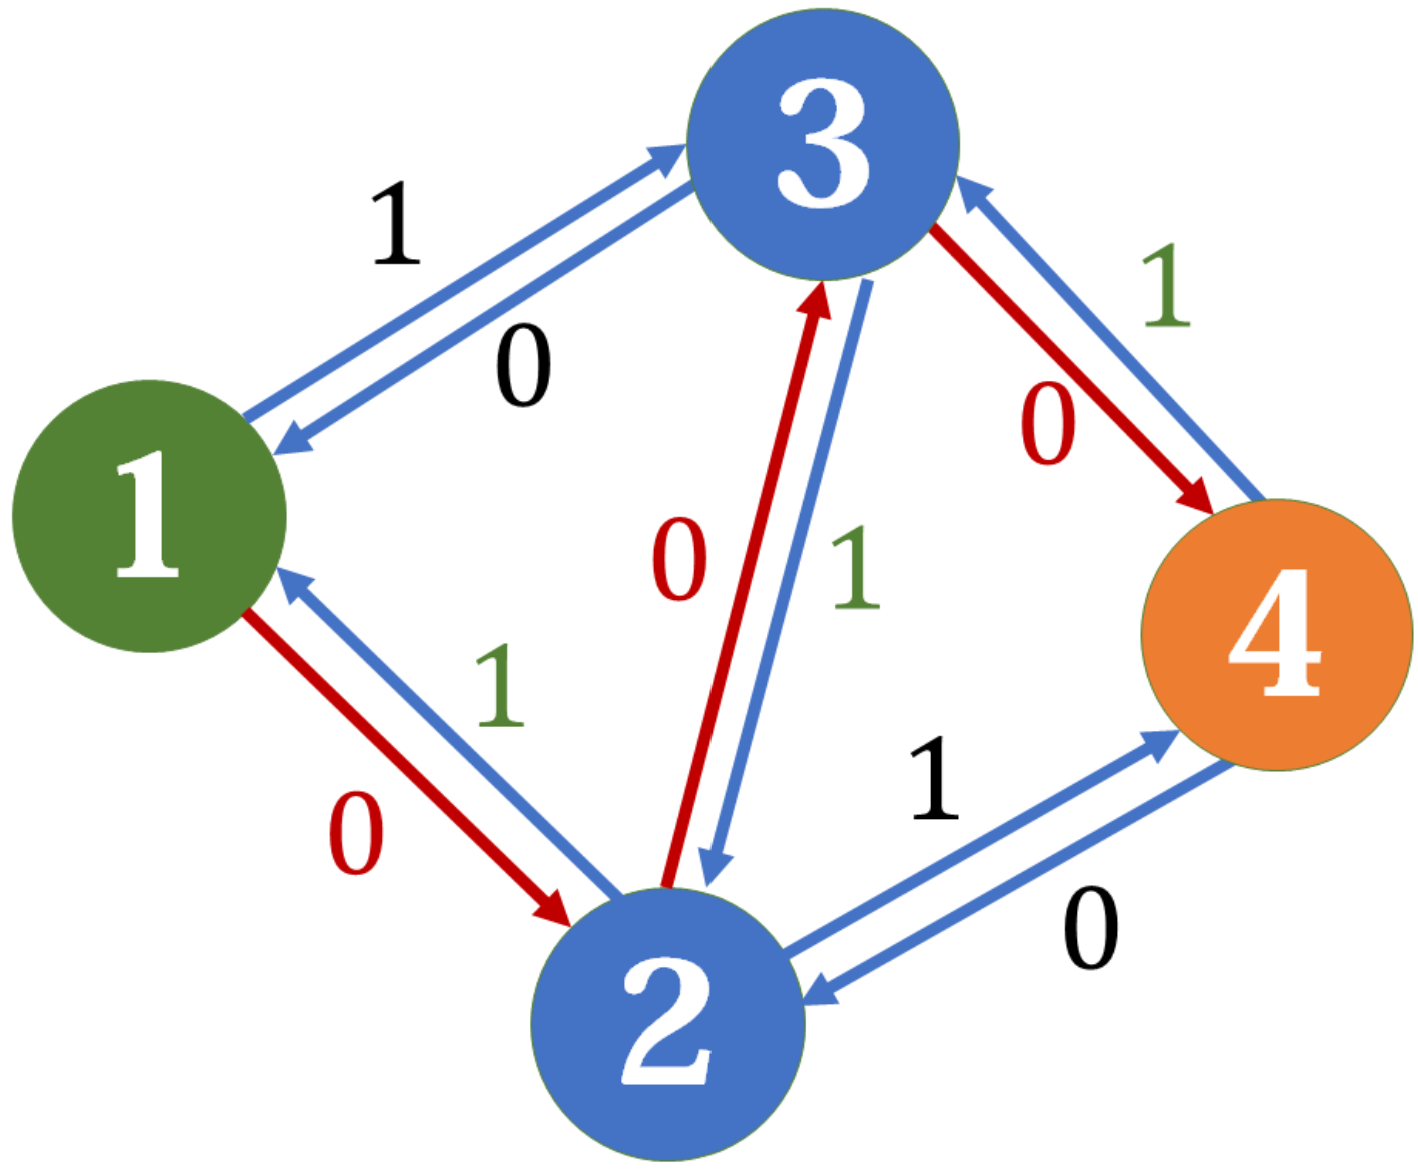
\includegraphics[width=0.3\textwidth]{maxflow2.png}
	% \caption{(1)}
	% \label{fig:example}
\end{figure}
\noindent 此时选择增广路 $(1,2,3,4)$ 和 $(1,3,2,4)$,$|f|=2$,边 $(2,3)$ 与其反边相互抵消,等价于选择增广路 $(1,3,4)$ 和 $(1,2,4)$。因此,加入反悔意味着 $G_f$ 中的每条可能的增广路都可以被访问,与访问顺序无关。对于反向边的存储,采用链式前向星和成对变换的技巧,即将每条边与它的反向边按编号连续存储,分别为 $k$ 和 $k\oplus1$,满足 $2\mid k$。
\subsubsection{最大流最小割定理}
\begin{mdframed}[leftline=true, linewidth=2pt, linecolor=gray]
	证明:对于给定有源汇网络,其最大流等于最小割,即 $|f|=\|S,T\|$。
\end{mdframed}
上述贪心的正确性证明和对最大流最小割定理的证明等价。\\
首先有引理:对于给定网络 $G$,任取一个流 $f$ 和一个割 $\{S,T\}$,总是有 $|f|\le||S,T||$,等号成立当且仅当所有 $S$ 到 $T$ 的割边为满流且所有 $T$ 到 $S$ 的割边为空流,证明如下:
\begin{align*}
	|f| &= f(s) \\
	&= \sum_{u \in S} f(u) \\
	&= \sum_{u \in S} \left( \sum_{v \in V} f(u,v) - \sum_{v \in V} f(v,u) \right) \\
	&= \sum_{u \in S} \left( \sum_{v \in T} f(u,v) + \sum_{v \in S} f(u,v) - \sum_{v \in T} f(v,u) - \sum_{v \in S} f(v,u) \right) \\
	&= \sum_{u \in S} \left( \sum_{v \in T} f(u,v) - \sum_{v \in T} f(v,u) \right) 
	+ \sum_{u \in S}\sum_{v \in S} f(u,v) - \sum_{u \in S}\sum_{v \in S} f(v,u) \\
	&= \sum_{u \in S} \left( \sum_{v \in T} f(u,v) - \sum_{v \in T} f(v,u) \right) \\
	&\le \sum_{u \in S}\sum_{v \in T} f(u,v) (empty)\\
	&\le \sum_{u \in S}\sum_{v \in T} c(u,v) (full)\\
	&= \|S, T\|
\end{align*}
回到原定理,假设某一轮增广后得到流 $f$ 使得 $G_f$ 上不存在增广路,此时记 $G_f$ 上从 $s$ 出发可以到达的点集为 $S$,$T=\mathbf{V}-S$,显然 $\{S,T\}$ 为 $G$ 的一个割(源汇点不连通)。\\
在残量网络上讨论,此时不存在从 $S$ 到 $T$ 的割边,所以有:
\begin{equation*}
	\forall u\in S,\forall v\in T,c_f(u,v)=0
\end{equation*}
将这些边分为存在于原图中的边和反向边两种情况讨论:
\begin{itemize}
	\item $(u,v)\in\mathbf{E}$,此时 $c_f(u,v)=0$,有 $c(u,v)=f(u,v)$,满流;
	\item $(v,u)\in\mathbf{E}$,此时 $c_f(u,v)=c(u,v)-f(u,v)=f(v,u)=0$,空流。
\end{itemize}
从而流函数 $f$ 满足引理的取等条件,为最大流,贪心正确,又任意流小于任意割,反证得此时 $\{S,T\}$ 为最小割,最大流最小割定理成立。
\subsubsection{Edmonds–Karp算法}
EK算法使用BFS求 $G_f$ 中的最短增广路并应用上述贪心,其时间复杂度为 $O(|\mathbf{V}||\mathbf{E}|^2)$。\\
% 省略对于其时间复杂度的证明,直到笔者看懂为止。
\subsubsection{Dinic/ISAP算法}
Dinic算法的核心思想是分层图以及相邻层之间增广,从而批量处理增广路。考虑增广前对 $G_f$ 做BFS分层,记结点 $u$ 的层数为 $\operatorname{lev}(u)$,对于 $\forall u\in G_f$,暂时删除残量网络中所有满足 $\operatorname{lev}(u)\ge\operatorname{lev}(v)$ 的边 $(u,v)$,形成DAG。此时分层图称为层次图,记为:
\begin{equation*}
	G_L=(\mathbf{V},\mathbf{E}_L),\mathbf{E}_L=\{(u,v)|(u,v)\in\mathbf{E}_f,\operatorname{lev}(u)+1=\operatorname{lev}(v)\}
\end{equation*}
此时层次图中所有的增广路均为最短增广路,使用DFS遍历所有的增广路,满足批量求增广路的需求。记增广流为对若干条增广路增广后得到的流,如果在 $G_L$ 上找到一个极大的增广流 $f_b$ 使得 $G_L$ 上不存在 $|f'|\ge|f_b|$,称 $f_b$ 为 $G_L$ 的阻塞流,将其累加进 $f$。\\
将以上过程称为一次分层,重复此过程直到新的 $G_L$ 中不存在增广路,即源汇点不连通,此时 $f$ 为最大流。注意,在一次分层中删除的边集 $\mathbf{E}'=\mathbf{E}_f-\mathbf{E}_L$ 在之后的分层中可能还会用到,这种删除等价于在DFS过程中忽略边集 $\mathbf{E}'$。\\
\\
注意到在 $G_L$ 上DFS时,如果结点 $u$ 同时具有大量入边和出边,并且 $u$ 每次接受来自入边的流量时都遍历出边表来决定将流量传递给哪条出边,则局部时间复杂度最坏可达 $O(|\mathbf{E}|^2)$。为避免这一缺陷,如果某一时刻已知边 $(u, v)$ 已经增广到极限,即边 $(u, v)$ 已无剩余容量或 $v$ 的后侧已增广至阻塞,则 $u$ 的流量没有必要再尝试流向出边 $(u, v)$。据此,对于每个结点 $u$,维护 $u$ 的出边表中第一条还有必要尝试的出边/指针,称其为当前弧,下一次DFS从当前弧开始遍历所有出边,跳过所有不可行边,称这个做法为当前弧优化,是算法不可或缺的一部分。Dinic算法总的时间复杂度为 $O(|\mathbf{V}|^2|\mathbf{E}|)$。
% 省略对于其时间复杂度的证明,直到笔者看懂为止。

\subsubsection{预流推进算法}

\newpage
\subsection{最小割树}
\begin{mdframed}[leftline=true, linewidth=2pt, linecolor=gray]
	将 $\mathbf{V}$ 分成互不相交的两个点集 $S,T$,当 $u\in S,v\in T$ 时将该割称为关于 $u,v$ 的割,记为 $\{u,v\}$。称 $\{u,v\}$ 的最小割为所有关于 $u,v$ 的割中容量最小的割,记为 $\|u,v\|$。给定一张带非负权的 $n$ 阶无向图,边数为 $m$,有 $q$ 个询问,每个询问给定一个非负整数 $x$,求图中有多少个无序点对的最小割的容量不超过 $x$。
\end{mdframed}
首先新建一张无边 $n$ 阶无向图 $G'$,然后在原图 $G$ 中任意选两个点 $s,t$,求出其最小割 $c=\|s,t\|$,并在 $G'$ 中在 $s,t$ 之间连一条边权为 $c$ 的无向边。递归地在 $s$ 所属的点集和 $t$ 所属的点集中重复上述过程,直到当前集合中只剩一个点。这个过程所构建的新图 $G'$ 为一棵树,称为最小割树,树上任意两个点在原图中的对应点之间的最小割值等于这两个点的树上路径中边权的最小值,下面证明该结论:\\
\\
回到原题,预处理出最小割树后,问题转化为:给定一颗 $n$ 阶非负权无根树,定义两点之间的距离为两点之间路径中的最小边权,每个询问给定非负整数 $x$,求距离小于等于 $x$ 的无序点对数量。考虑Kruskal重构树:将边权后放入大根堆,然后依次取出,在并查集上合并每条边两边端点所在的集合,并维护集合大小。设合并的两点 $\{x,y\}$ 所在的集合大小为 $s_x,s_y$,则有 $s_x\times s_y$ 个无序点对的距离为该边边权。设距离为 $w$ 的无序点对数量总共有 $p_w$ 个,则对于每次询问,通过在 $p$ 对应的前缀和数组上二分得到答案。总的时间复杂度为 $O(n^3m+n\log{n}+q\log{n})$。

\subsection{有界流} % 上下界网络流
\subsection{费用流}
\begin{mdframed}[leftline=true, linewidth=2pt, linecolor=gray]
	给定网络 $G=(\mathbf{V},\mathbf{E},c,w)$,若单位流量费用 $w(u,v)$ 也满足斜对称性,则将网络中总花费 $f\times w$ 最小的最大流称为最小费用最大流,即最大化 $|f|$ 的前提下最小化 
	\begin{equation*}
		\sum_{(u,v)\in\mathbf{E}}f(u,v)\times w(u,v)
	\end{equation*}
\end{mdframed}
\subsubsection{SSP算法}
\subsubsection{Primal-Dual算法}
\subsubsection{zkw费用流}
\subsubsection{带负圈费用流}
\subsection{线性规划}
\newpage
\section{二分图}
\section{序理论}
\subsection{基本定义}
\subsection{拓扑排序}
\subsection{Dilworth定理}
\newpage
\section{树论基础}
\subsection{树的遍历}
\subsection{树的直径}
\subsection{树的中心}
\subsection{树的重心}
\subsection{最近公共祖先}
\subsubsection{倍增算法}
\subsubsection{欧拉序}
\subsubsection{DFS序}
\subsubsection{树链剖分}
\subsection{树上差分}
\newpage
\section{树链剖分}

\newpage
\part{线性代数}
\section{线性基}
\subsection{定义与性质}
称代数系统 $<V,+,\cdot,\mathbf{P}>$是 $V$ 关于 $+,\cdot$ 构成 $\mathbf{P}$ 上的线性空间,$\mathbf{P}$ 为线性空间的基域,$V$ 中元素称为向量,$\mathbf{P}$ 中的元素称为标量。$V$ 的一个极大线性无关组为一组线性基,简称基。记 $\theta$ 为加法群的零元,规定线性空间 $\{\theta\}$ 的基为空集。可以证明任意线性空间均存在线性基,定义线性空间 $V$ 的维数为线性基的元素个数,记作 $\dim V$。\\
\\
线性基具有如下性质:
\begin{enumerate}
	\item 对于有限维线性空间 $V$ (可以推广至无限线性空间),设 $n=\dim V$,则:
	\begin{itemize}
		\item $V$ 中的任意 $n+1$ 个向量线性相关;
		\item $V$ 中任意 $n$ 个线性无关的向量均为 $V$ 的基;
		\item 若 $V$ 中任意向量均可被向量组 $(a_1,a_2,...,a_n)$ 线性表示,则其是 $V$ 的一个基;
		\item $V$ 中任意线性无关向量组均可通过插入若干向量使得其成为 $V$ 的一个基。
	\end{itemize}
	\item 令 $V_1,V_2$ 是关于 $\mathbf{P}$ 的有限维线性空间,且 $V_1+V_2,V_1\bigcap V_2$ 也是有限维的,则:
	\begin{itemize}
		\item $\dim V_1+\dim V_2=\dim (V_1+V_2)+\dim(V_1\bigcap V_2)$;
		\item 若 $(a_1,...a_n)$ 是 $V_1$ 的一组基,$(b_1,...b_m)$ 是 $V_2$ 的一组基,则 $(a_1,...a_n,b_1,...b_m)$ 是 $V_1+V_2$ 的一组基。
	\end{itemize}
\end{enumerate}
从而通过线性基可以实现如下功能:
\begin{enumerate}
	\item 求给定向量组的秩;
	\item 对给定的向量组,找到一组极大线性无关组(或其张成的线性空间的一组基);
	\item 向给定的向量组插入某些向量,在插入操作后的向量组中找到一组其张成的线性空间的一组基;
	\item 对找到的一组基,判断某向量能否被其线性表出;
	\item 对找到的一组基,求其张成的线性空间中的特殊元素(如最大元、第 $k$ 小元等)。
\end{enumerate}

\newpage
\subsection{异或线性基}
一般将 $n$ 维布尔域线性空间下 $\mathbf{Z}_2^n$ 的线性基称为异或线性基,可以证明代数系统 $<\mathbf{Z}_2^n,\oplus,\And,\mathbf{Z}_2>$ 是线性空间。\\
回到原题,可以根据给定的 $m$ 个数所转化的布尔序列 $X=\{x_1,...x_m\}$ 构建一组异或线性基 $B=\{b_1,...b_n\}$,满足如下性质:
\begin{enumerate}
	\item $B$ 中任意非空子集异或和不为 $0$;
	\item 对 $X$ 中任意元素都可以表示为 $B$ 中若干元素的异或和;(数乘为与且域 $\mathbf{Z}_2$ 中元素为 $\{0,1\}$)
	\item 对任意满足以上两条的集合 $B'$,其元素个数不少于 $B$ 的元素个数。
\end{enumerate}
异或线性基可以实现如下功能:
\begin{enumerate}
	\item 判断一个数能否表示成某数集子集的异或和;
	\item 求一个数表示成某数集子集异或和的方案数;
	\item 求某数集子集的最大/最小/第 $k$ 大/第小 $k$ 异或和;
	\item 求一个数在某数集子集异或和中的排名。
\end{enumerate}
\subsubsection{最大异或和}
\begin{mdframed}[leftline=true, linewidth=2pt, linecolor=gray]
	给定 $m$ 个整数(数字可能重复),在这些数中选取任意个使得他们的异或和最大,求该最大异或和的值。
\end{mdframed}
有两种构造异或线性基的方法,消元法和贪心法。消元法即将 $m$ 个布尔序列构成二进制矩阵通过高斯消元法消成线性基。其步骤如下:
\begin{enumerate}
	\item 从高到低位枚举(等价于按列枚举)。
	\item 确定主元(某一行对应的值)。假设枚举到了第 $i$ 位,找到一个该位为 $1$ 的数,将其置换到第 $i$ 行。
	\item 对其他的数:假如该数第 $i$ 位为 1,那就让这个数异或主元,让这一位变成 0,否则不操作。
\end{enumerate}
例如对于序列 $\{7,5,9,2\}$,有如下行列变换:
\begin{align*}
\begin{bmatrix}0 & 1 & 1 & 1 \\0 & 1 & 0 & 1 \\1 & 0 & 0 & 1 \\0 & 0 & 1 & 0\end{bmatrix}\;\xrightarrow{\operatorname{swap}(R_1,R_3)}\;\begin{bmatrix}1 & 0 & 0 & 1 \\0 & 1 & 0 & 1 \\0 & 1 & 1 & 1 \\0 & 0 & 1 & 0\end{bmatrix}\;\xrightarrow{R_3=R_3\oplus R_2}\;\begin{bmatrix}1 & 0 & 0 & 1 \\0 & 1 & 0 & 1 \\0 & 0 & 1 & 0 \\0 & 0 & 1 & 0\end{bmatrix}\;\xrightarrow{R_4=R_4\oplus R_3}\;\begin{bmatrix}1 & 0 & 0 & 1 \\0 & 1 & 0 & 1 \\0 & 0 & 1 & 0 \\0 & 0 & 0 & 0\end{bmatrix}
\end{align*}
从而 $B=\{9,5,2\}$。易证$B$ 中元素严格递减,且二进制矩阵是一个行简化阶梯形矩阵。这意味着基中所有元素异或和即是最大异或和。\\
相较于消元法,贪心法可以做到在线插入元素并在线更新线性基。其过程如下:
\begin{enumerate}
	\item 令 $p$ 表示原序列的线性基数组,$p_i$ 表示第 $i$ 位的向量。初始时基为空集,$p_i=0,i\in[0,Bits]$;
	\item 当插入一个数 $x$ 时,从高到低位枚举 $x_{(2)}$,如果 $x_{(2)}$ 的第 $i$ 位是 $1$,判断 $p_i$ 是否存在:
	\begin{itemize}
		\item 若不存在则插入并退出,即 $p_i=x$;
		\item 否则将 $x$ 异或上 $p_i$ 并枚举 $x'_{(2)}$ 的下一位。
	\end{itemize}
\end{enumerate}
从而 $B=\{p_i\mid p_i\ne0\}$。例如对于序列 $\{7,5,9,2\}$,有如下插入操作:
\begin{align*}
	p_{3\rightarrow0} &=
	\begin{bmatrix}0 \\ 0 \\ 0 \\ 0\end{bmatrix}
	\xrightarrow{\operatorname{insert}(7),\,p_2=7}
	\begin{bmatrix}0 \\ 7 \\ 0 \\ 0\end{bmatrix}
	&\xrightarrow{\operatorname{insert}(5),\,p_1=2}
	\begin{bmatrix}0 \\ 7 \\ 2 \\ 0\end{bmatrix}
	&\xrightarrow{\operatorname{insert}(9),\,p_3=9}
	\begin{bmatrix}9 \\ 7 \\ 2 \\ 0\end{bmatrix}
	&\xrightarrow{\operatorname{insert}(2),\,p_0=0}
	\begin{bmatrix}9 \\ 7 \\ 2 \\ 0\end{bmatrix}
\end{align*}
假设存在 $i,j,k$ 使得 $p_i\oplus p_j\oplus p_k=0$,则 $p_k$ 不会被插入,从而 $B$ 中任意非空子集异或和不为 $0$ 且 $B$ 中元素不能被其他元素表出。\\
由异或性质,如果 $x\ne0$ 最终没有插入 $B$,则 $x\oplus \{p_i|x_i=1\}=0\Rightarrow\{p_i|x_i=1\}=x$,即基中若干元素可以异或出 $x$,从而原序列中的每一个数都可以通过线性基表出。\\
此外,$p_i\oplus p_j\oplus p_k=x\iff p_i\oplus p_j\oplus x=p_k$,即插入顺序会影响贪心法得出的基,又因为每个插入的数对应着一个二进制位,所以 $x$ 与 $p_k$ 相排斥只会影响一个元素,即线性基里的数可能不同,但是总数肯定是一定的。\\
贪心法求最大值时,需要对线性基求前缀最大值(从高到低位),即枚举到第 $i$ 位时,需要用前缀的异或最大值去异或 $p_i$,更新最大值。
\begin{lstlisting}
for(int i = Bits; i>= 0; i--) ans = max(ans, ans ^ p[i]);
\end{lstlisting}

\subsubsection{求第k小异或和}
\begin{mdframed}[leftline=true, linewidth=2pt, linecolor=gray]
	给由 $n$ 个数组成的一个可重集 $S$,每次给定一个数 $k$,求集合 $T \subseteq S$ 的异或和,其中集合 $T$ 满足: 在 $S$ 的所有非空子集的不同的异或和中,其异或和 $T_1 \oplus T_2 \oplus \ldots \oplus T_{|T|}$ 是第 $k$ 小的。$1\le n,m\le 10^5,0\le S_i,k\le2^{50}$
\end{mdframed}
若用贪心法得到 $S$ 的线性基 $B$,就再用消元法处理成 $B'$,使得基中任何一个二进制位至多有一个元素是 $1$,从而可以不重复使用任意一个元素就张成线性空间。\\
设 $k_{(10)}=(k_M...k_0)_{(2)},p_i\in B'$,则第 $k$ 小异或和为 $\displaystyle\sum_{i=0}^{Bits}k_i\cdot p_i$。原序列中有 $0$ 则 $k\leftarrow k-1$。

\newpage
\section{特征根}
\begin{mdframed}[leftline=true, linewidth=2pt, linecolor=gray]
	有一个 $1$ 行,$n+1$ 列的棋盘,编号为 $0$ 到 $n$。初始时刻,在位置 $m$ 有一颗棋子。如果某一秒棋子不位于 $n$,那么它将有 $p$ 的概率向左移动一格,$1-p$ 的概率向右移动一格;否则,棋子向左移动一格。求期望多少秒之后棋子能够到达$0$。答案对于$10^9+7$取模。$1\le m\le n\le 10^9$,保证 $p$ 和答案是有理数。
\end{mdframed}

设 $E_i$ 表示当棋子位于位置 $i$ 时期望走到 $0$ 的时间,则有 $n+1$ 个方程:
\begin{align*}
	E_i = 
	\begin{cases}
		0, & i = 0, \\[6pt]
		pE_{i-1}+(1-p)E_{i+1}+1, & 0 < i < n, \\[6pt]
		E_{n-1}+1, & i = n.
	\end{cases}
\end{align*}
考虑第 $i+1$ 个方程,变形得 
\begin{equation*}
	\displaystyle E_i-E_{i-1}=\frac{1-p}{p}(E_{i+1}-E_i)+\frac{1}{p}
\end{equation*}
令 $F_i=E_i-E_{i-1}$,则 $\displaystyle F_i=\frac{1-p}{p}F_{i+1}+\frac{1}{p}, E_x=\sum_{i=1}^{x}F_i$ ,根据特征根法得出通项公式为: 
\begin{equation*}
	\displaystyle F_i=(\frac{1-p}{p})^{n-i}(F_n+\frac{1}{1-2p})-\frac{1}{1-2p} , F_n=1,p\ne\frac{1}{2}
\end{equation*}
当 $\displaystyle p\ne\frac{1}{2}$ 时,这是等比数列求和,否则 $F_i=F_{i+1}+2$,为等差数列求和。\\

特征根就是矩阵的特征方程的解,考虑构造伴随矩阵并利用矩阵快速幂求解 $E_i$。对于第 $i+1$ 个方程,变形得带常数的齐次线性递推式 \begin{equation*}
	\displaystyle E_{i+1}=\frac{1}{1-p}E_{i}-\frac{p}{1-p}E_{i-1}-\frac{1}{1-p},p\ne1
\end{equation*}
令 $v_{n+1}=Mv_n\Rightarrow v_n=M^{n-1}v_1$,有
\begin{align*}
	\displaystyle v_i&=\begin{bmatrix}E_i\\E_{i-1}\\1\end{bmatrix},v_1=\begin{bmatrix}E_1\\0\\1\end{bmatrix},M=\begin{bmatrix}\frac{1}{1-p} & -\frac{p}{1-p} & -\frac{1}{1-p}\\1 & 0 & 0\\0 & 0 & 1\end{bmatrix}
\end{align*}
通过 $E_n=E_{n-1}+1$ 解出 $E_1$,继而求出 $E_m,1\le m\le n$。注意取模和对应的乘法逆元。
当 $p=1$ 时 $E_i=E_{i-1}+1$。

\newpage
\part{抽象代数}

\newpage
\part{组合数学}

\newpage
\part{计算几何}

\newpage
\part{概率论}

\newpage
\part{博弈论}
\section{公平组合博弈}
\subsection{基本定义}
公平组合博弈(Impartial Game)指的是满足如下条件的博弈:
\begin{itemize}
	\item 两个玩家交替行动、信息完全、没有概率成分、局面有限且终局明确的博弈(组合博弈);
	\item 在任意确定状态下,所有参与者可选择的行动完全相同,仅取决于当前状态,与身份无关(公平博弈);
	\item 博弈中的同一个状态不可能多次抵达,博弈以参与者无法行动为结束,且博弈一定会在有限步后以非平局结束(非反常博弈);
	\item 交换两个玩家的身份,收益函数不变(对称博弈)。
\end{itemize}
在一个公平组合游戏中,每个玩家是否有必胜策略,只取决当前游戏所处的状态而与玩家的身份无关。因此,所有状态可以分为先手必胜状态 和先手必败状态,分别记为 $\mathcal N$ 态和 $\mathcal P$ 态。这个定义适用于所有公平组合游戏,从而可以归纳地将正常规则的公平组合游戏中所有状态标记为必胜状态和必败状态:
\begin{itemize}
	\item 没有后继状态的状态是必败状态 $\mathcal P$;
	\item 一个状态是必胜状态 $\mathcal N$ 当且仅当存在至少一个它的后继状态为必败状态 $\mathcal P$;
	\item 一个状态是必败状态 $\mathcal P$ 当且仅当它的所有后继状态均为必胜状态 $\mathcal N$。
\end{itemize}

\newpage
\subsection{简单Nim游戏}
\begin{mdframed}[leftline=true, linewidth=2pt, linecolor=gray]
	共有 $n$ 堆石子,第 $i$ 堆有 $a_i$ 枚石子。两名玩家轮流取走任意一堆中的任意多枚石子,但不能不取。取走最后一枚石子的玩家获胜。判断先手是否必胜。
\end{mdframed}
容易验证,Nim 游戏是正常规则的公平组合游戏,其局面/状态(双方玩家过往的行动、已经实现的随机变量值、双方已知信息的内容等)可能的变化可以用博弈图来描述:将每一个可能的状态都看作是图中的一个结点,并将状态向它的后继状态(即通过一次操作可以达到的状态)连边,得到一个有向无环图。博弈图是无环的,因为 Nim 游戏中,每次操作,石子的总数量都是严格减少的。例如,对于初始局面有 $3$ 堆石子,且每堆石子的数量分别为 $1,1,2$ 的 Nim 游戏,可以绘制如下的博弈图:
\begin{figure}[H]
	\centering
	% \raggedright
	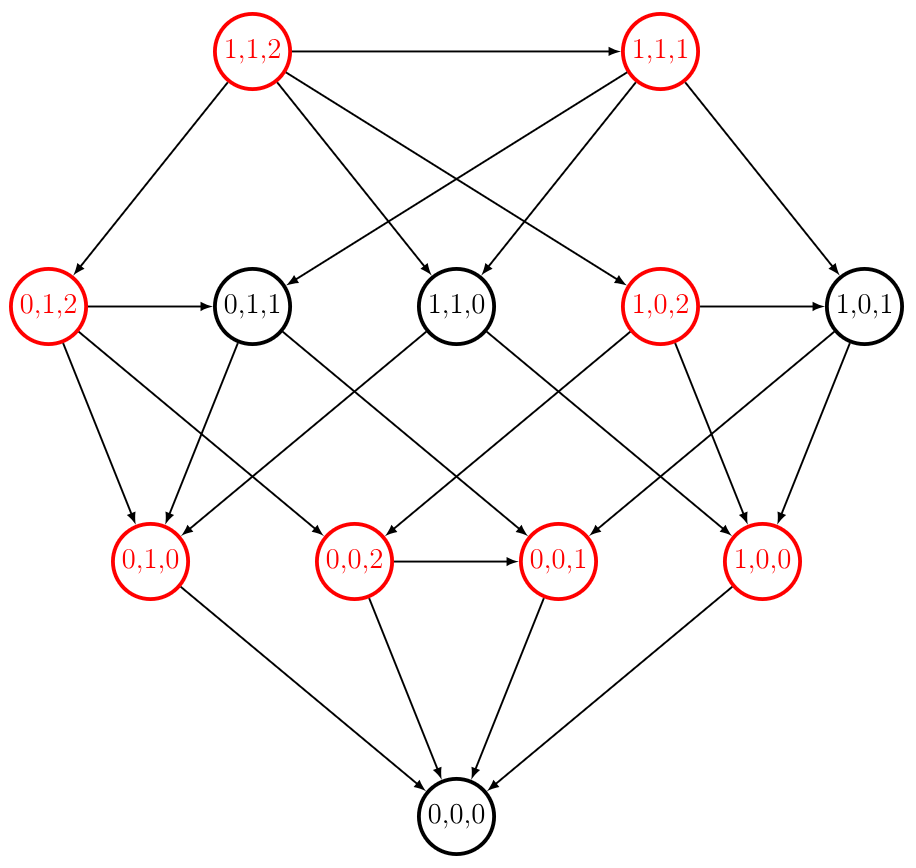
\includegraphics[width=0.4\textwidth]{game1.png}
	% \caption{(1)}
	% \label{fig:example}
\end{figure}
\noindent 其中红色结点表示必胜状态,黑色结点表示必败状态。\\
假设在某一时刻第 $i$ 堆有 $A_i(0\le A_i\le a_i)$ 枚石子,定义其Nim和为 $k=A_1\oplus A_2\cdots\oplus A_n$,其状态为必败状态 $\mathcal P$ 当且仅当Nim和为 $0$,证明如下:
\begin{enumerate}
	\item 如果对于 $\forall i\in[1,n],A_i=0$,则该状态没有后继状态,且 $k=0$,命题成立。
	\item 如果 $k\ne0$,构造一个合法移动,使得后继状态为必败状态:由归纳假设,只需要证明存在后继状态满足 $k'=0$ 即可。设 $k$ 的二进制表示中,最高位的 $1$ 是第 $d$ 位,则一定存在某个 $A_i$,使得其二进制第 $d$ 位是 $1$。对于相应的石子堆,一定有 $A_i>A_i\oplus k$。考虑将该石子堆减到 $A'_i=A_i\oplus k$,此时 $k'=A_1\oplus\cdots A'_i\oplus\cdots\oplus A_n=k\oplus k=0$。
	\item 如果 $k=0$,需要证明该状态是必败状态。由归纳假设可知,只要证明它的所有后继状态的 Nim 和都不是 $0$。这是必然的,任何合法移动将 $A_i$ 变为 $A'_i\neq A_i$,都会使 $k'=k\oplus A_i\oplus A'_i\ne0$。
\end{enumerate}
\subsection{Sprague–Grundy理论}
SG理论指出,所有公平组合游戏都等价于单堆Nim游戏。当游戏由若干个相互独立的子游戏组成时,游戏的状态判定可以通过计算子游戏的SG函数值的Nim和来完成。

\newpage
\part{多项式}

\newpage
\part{字符串}

\newpage
\part{数据结构} % 包含离线算法
\section{单调栈 }% 包含悬线法
\section{单调队列}
\section{链表} % 包含DLX
\section{可并堆} % 包含左偏树
\section{斐波那契堆}
\section{哈希表} % 包含离散化
\section{并查集}
\section{ST表}
\section{树状数组}
\section{线段树}
\section{平衡树}

\newpage
\part{动态规划}
\section{背包DP} % 见pack.pdf

\newpage
\part{其他科技}
\section{均摊分析}
\section{计算理论}  % 包含自动机
\subsection{自动机}
\subsection{形式语言}
\subsection{可计算性}
\subsection{复杂性理论}
\section{查找算法}
\subsection{二分/三分}
\subsection{分数规划}
\subsection{双指针}
\section{信息论}
\section{随机化算法}
\end{document}
